\documentclass[11pt]{article}

\usepackage[english]{babel}
\usepackage[utf8]{inputenc}
\usepackage{amsmath}
\usepackage{graphicx}
\usepackage[colorinlistoftodos]{todonotes}
%\usepackage[margin=1in]{geometry}
\usepackage{listings}
\usepackage{hyperref}
\usepackage{units}
\usepackage[margin=0.75in]{geometry}
\title{E155 Final Report}

\author{Cindy Angpraseuth, Rachel Roley}

\date{\today}

\begin{document}
\maketitle

\section{Introduction}

%The aim of this project is to create an interactive lightsaber that will respond to the user's movements. The blade of the sword will be made of a clear material, with an LED strip embedded inside that will make the lightsaber appear to glow.  The color of the LEDs is controlled with a potentiometer.  Depending on how forcefully a user swings the lightsaber, different sounds will play. This data will be measured using an IMU. The following sections detail the design process, and the progress made. 

The aim of the project is to create an interactive light saber that will respond to the user's movements. Current progress on the project is detailed in the following sections and summarized here. Overall, the final project will operate as shown in the block diagram in Figure \ref{fig:block}. Values will be read from a potentiometer using the PIC's ADC to toggle the color of a LED strip communicating over SPI. The FPGA will receive data from an IMU via SPI and use internal logic to determine "noise coefficients." These coefficients will be transmitted to the PIC32 over SPI, where they will be used to determine the relative proportion of a set of sine waves representing different lightsaber noises. These waves will be added and output to a DAC, which will send the sound wave to the speaker.  

Currently, we are able to read from a potentiometer using the PIC's ADC and display the value read on the board's LEDs. Additionally, we can communicate with the LED strip using SPI, and display a chosen color. We have also constructed several sine waves representing lightsaber noises on the PIC, and constructed the audio amplifier and DAC circuit. Future work will focus on the FPGA and IMU. 


\begin{figure}[h!]
\centering
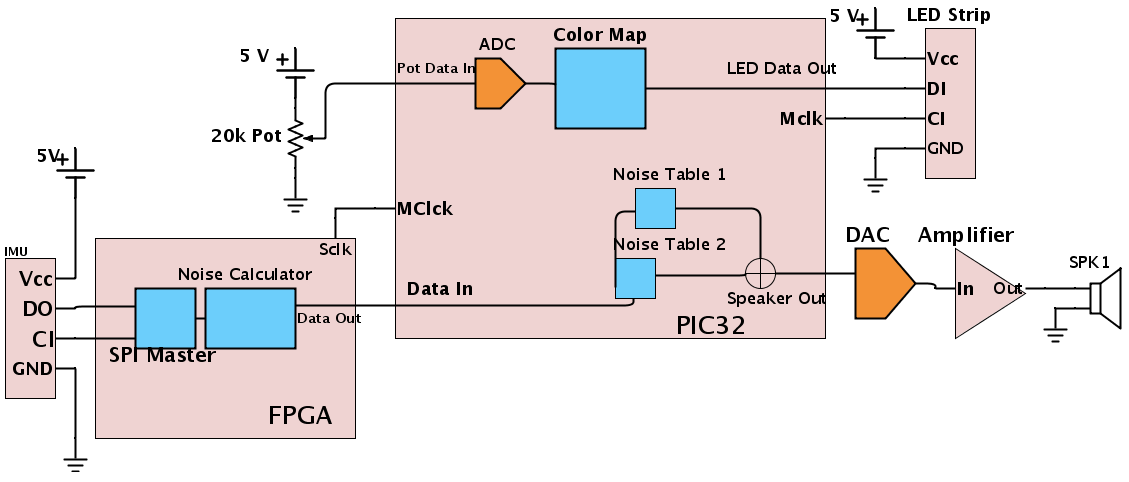
\includegraphics[width=1\textwidth]{SystemDiagram2.png}
\caption{\label{fig:block}} An overall block disgram of the system.
\end{figure}

\section{Sound Effects}

% \subsection{Audio Amplifier}
% \begin{figure}[h!]
% $$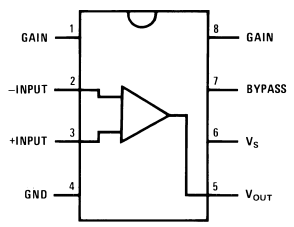
\includegraphics[width=0.3\textwidth]{LM386} \hspace{0.1\textwidth} 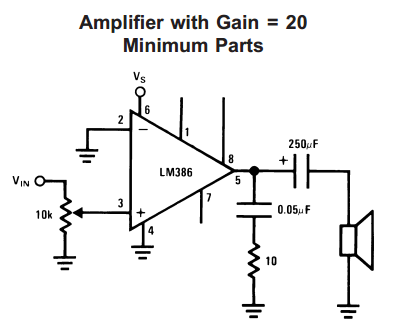
\includegraphics[width=0.4\textwidth]{ampMinParts}$$
% \caption{Left: pinout of LM386, Right: circuit diagram for LM386 and speaker}
% \label{fig:LM386}
% \end{figure}

Some debugging remains to be done in the sound effect implementation. So far, only a background hum has been programmed.  Once successful, the rest of the sound effects should follow easily.

\subsection{Audio Circuit}

Below in Figure \ref{fig:audioCircuitDiagram} is a diagram of the audio circuit.  The digital output from the PIC goes to a digital to analog converter.  From there, the signal is sent through an op amp to the speaker.

 \begin{figure}[h!]
 $$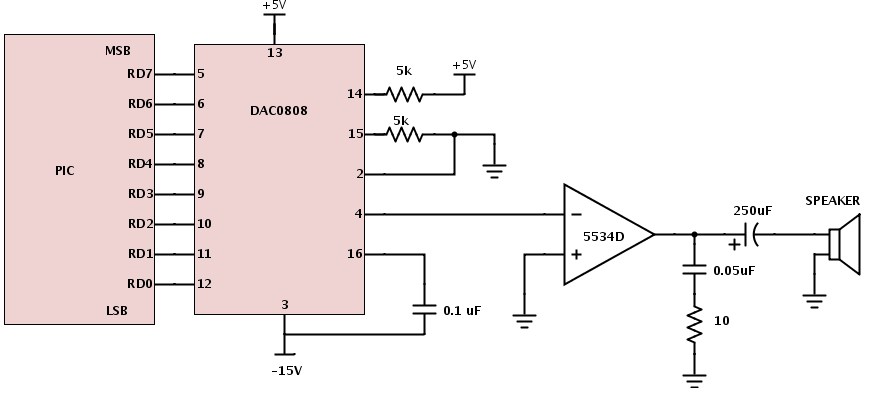
\includegraphics[width=0.8\textwidth]{audioCircuitDiagram}$$
 \caption{Circuit diagram of the digital audio output from the PIC to the speaker}
 \label{fig:audioCircuitDiagram}
 \end{figure}

\subsection{Audio Signal}
A YouTube video of lightsaber sound effects was downloaded and and the mp3 file was opened in Audacity. The desired sound effects were isolated and the sampling rate was decreased from the original 48 kHz.  In the case of the background hum, a sampling rate of 1 kHz was chosen. The data points of the sound wave were output as a csv file.

The values output by audacity range from -1 to 1, with up to 5 (decimal) significant figures.  Since the DAC output has 8 binary bits of resolution, the values must be rescaled.  The range of positive and negative numbers will be expressed in two's complement, which means that a range of integers from -128 to 127 (decimal) can be expressed.  The rescaling can be done using the following formula \cite{scalingFormula}:

$$f(x) = \frac{(b-a)(x-\text{min})}{\text{max}-\text{min}} + a$$

Where [min, max] is the original range and [a,b] is the desired range.  Microsoft Excel was used to do this conversion and round to the nearest integer.
% If the input is a float and the output is an int, I can express the output with 8 binary bits.


\subsection{Audio PIC Code}

The converted data points were put into a header file called backgroundHum.h, similar to the notes.h header file in Lab 5.  A value of 200 was added as the last data point, an arbitary choice outside of the -128 to 127 range, to mark the end of the audio file.  An index was initialized to step through the header file.  TRISD and PORTD were set to 0 so the digital audio output could be written to the same port as the LEDs for debugging.  Timer 1 was initialized on the PIC with a prescalar of 256. Assuming a peripheral clock at 5 MHz, the timer should increment at a frequency of approximately 19.5 kHz.  Since the sampling frequency was 1 kHz, a while loop checked whether TMR1 \% 20 is 0.  If it was, the value from the header file was sent to PORTD and the index was incremented to be ready for the next value. If the value was 200, the break in the loop occured. 

In future work, the mod operator will be replaced. Since the code takes time to run, it is possible that the lag will cause the if statement to always return false because the timer is not divisible by 20 every time it is checked.
%leave as a comment? seems informal
%(NOTE: I am realizing as I write this report that I should not have used the mod operator.  Since the code takes time to run, it's possible that the timer will never be divisible by 20 when it is checked.)




 
%  In Figure \ref{fig:audioCircuit} is the physical counterpart to the circuit diagram in Figure \ref{fig:audioCircuitDiagram}.
 
%   \begin{figure}[h!]
%  $$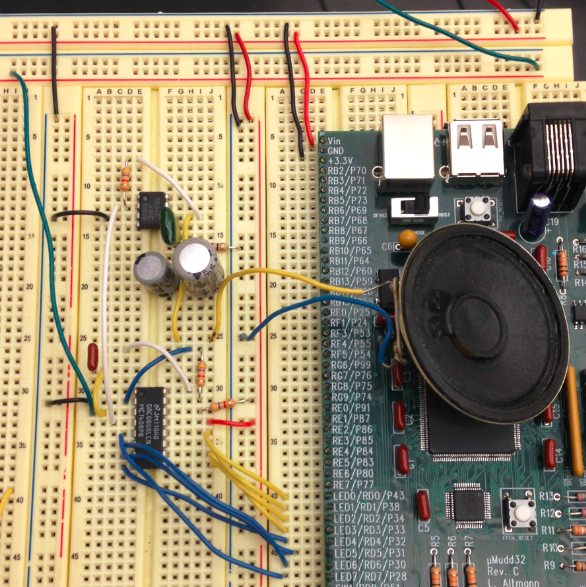
\includegraphics[width=0.4\textwidth]{audioCircuit}$$
%  \caption{Physical audio circuit}
%  \label{fig:audioCircuit}
%  \end{figure}

\section{LED Strip}

\subsection{Potentiometer Control}
The value of a 20k linear potentiometer connected to 5V and ground is read in using the PIC's built in ADC \cite{Section17ADC}. The code, detailed in the appendix, has two main functions which deal with the ADC converter: initadc() and readadc(). Initadc() will initial the analog to digital converter by setting up parameters. The most relavent parameters are the channel which is being used to take the analog voltage as input. Currently the code sets RB7 as the input, and configures the entire set of RB pins as either digital or analog. In future iterations of the project, greater care will be taken to this configuration. This is because one of the SPI clocks, SCK3, shares a pin with RB14, which is currently configured. The connections can be seen in Figure \ref{fig:adc}.


\begin{figure}[h!]
\centering
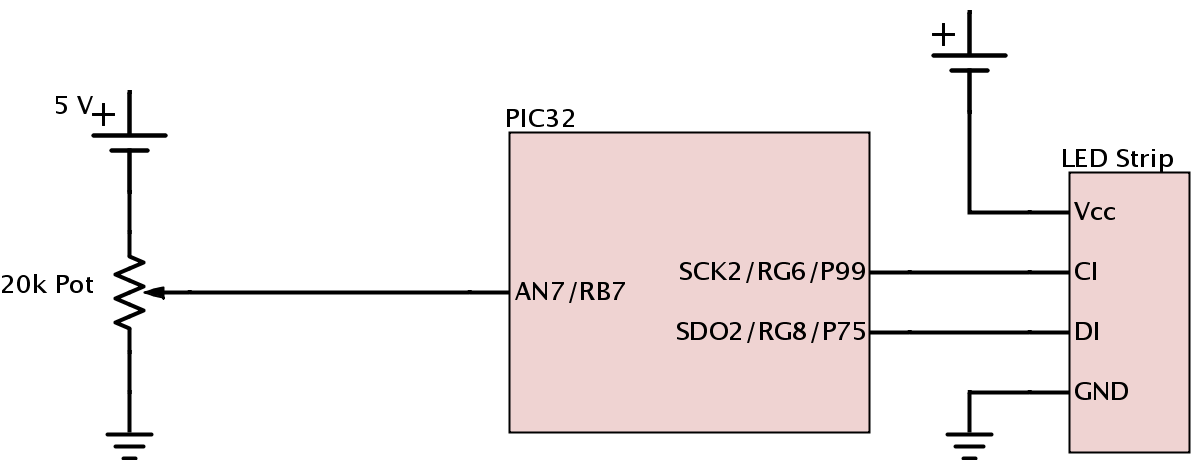
\includegraphics[width=.75\textwidth]{ledsys.png}
\caption{\label{fig:adc}} A simple circuit diagram of the LED circuit. 
\end{figure}

Readadc() takes a single sample, and returns it. Currently, this sample is written to the LEDs written on the board, allowing a user to ensure that the ADC is working. By turning the potentiometer, it is possible to see the numbers displayed on the LEDs transition bit by bit from 0 to 127 (111111), corresponding to 0V to 5V. Currenrtly, these LEDs are only being used for debugging purposes. In future iterations of the design, the ADC values will be mapped to RGB values. In this way, a user will be able to slowly transition through a rainbow of color using the potentiometer.


\subsection{LED Strip Characteristics}
The LED strip used for this project allows the user to set the color of each individual LED. The strip itself consists of a string of LEDs, controlled by a LPD8806 chip on a flexible circuit board. The module uses SPI communication. The system uses a latch based communication protocol: the first data out will be sent to the LED nearest to the controller, the second LED to the second nearest, and so on until all the LEDs at the end of the strip are illuminated. As soon as one driver has received the 32 bits of expected data, it passes all subsequent bytes until a latch condition takes place. This latching does not happen in unison, but  rather at the rate of data arrvial. 

In order to set an LED, a 32 bit number representing the green, red, and blue componenets of the desired color should be sent over the "Data In" pin to the strip. The color bytes expect the most significant bit set to high, with the remaining 7 bits set as a color brightness value. This can express numbers from 0 to 127.

\subsection{SPI Communication}
In order to allow for SPI communication, the strip is connected as shown in Figure \ref{fig:adc}.

Within the code attached in the appendix, the relavent functions are initSPI() and spiout(). InitSPI() initializes the communication of the PIC with the LED strip, setting the appropraite configuration bits. In order to reach the desired 2 MHz speed for sck needed for the LED strip, with a peripheral clock of 40 MHz/2, SPI2BRG is calculated by \cite{Section23SPI}:

\begin{align*}
F_{Sck} = \frac{F_{pb}}{2(SPI2BRG +1 )} \\
\unit[2]{MHz} = \frac{\unit[20]{MHz}}{2(SPI2BRG +1 )}
\end{align*}

In addition to setting the data rate, spiout() and show() handle the output of data and the LED indexig respectively. SpiOut() simply fills the SPI buffer with a 32 bit output. Show() will, when given an LED index, will find the color desired for that index and send it over SPI. 

\subsection{Setting Colors}
Focused in the functions Color(r,g,b), setPixelColor(n,color), and colorWipe(color), there are a number of steps involed in setting an LED a given color. First, a 32-bit color value is created. Given a r,g,b user input, the function will make sure the first bit, reserved for data transmission signaling, is 1. It will combine the three 8 bit numbers into a single 32 bit number which the LED driver will understand. setPixelColor() will take in this color number, as well as an LED index. Using the array of pixel colors, it will assign a color to the desired LED in the array. This array is later referenced in colorWipe, which takes in a single color and loops over all of the LEDs, setting them the desired color and using show to reference that color and display them.  


\section{Bill of Materials}

\begin{table}[h!]
\centering
\begin{tabular}{|l|l|l|l|}
\hline
Name                       & Part Number/Value       & Vendor        & Price   \\ \hline
IMU                        & LSM9DS0                 & Adafruit      & \$24.95 \\ \hline
Digital RGB LED Strip (1m) & LPD8806                 & Adafruit      & \$29.95 \\ \hline
Clear PETG Tube (2ft)      & 9245K51                 & McMaster Carr & \$13.78 \\ \hline
Speaker                    & N/A                     & E155 Lab      & N/A     \\ \hline
DAC                        & DAC0808LCN              & Stockroom     & N/A     \\ \hline
Op Amp                     & 5534D JRD               & Stockroom     & N/A     \\ \hline
Potentiometer              & 20 kOhms                & Stockroom     & N/A     \\ \hline
Assorted Resistors         & 10 Ohms, 5 kOhms        & Stockroom     & N/A     \\ \hline
Assorted Capacitors        & 0.05 uF, 0.1 uF, 250 uF & Stockroom     & N/A     \\ \hline
\end{tabular}
\caption{Bill of Materials}
\end{table}

\pagebreak

\begin{thebibliography}{99}
\bibitem{scalingFormula}
\url{http://stackoverflow.com/questions/5294955/how-to-scale-down-a-range-of-numbers-with-a-known-min-and-max-value}
\bibitem{Section17ADC}
\url{http://ww1.microchip.com/downloads/en/DeviceDoc/61104E.pdf}
\bibitem{SampleCode} 
\url{https://github.com/adafruit/LPD8806/blob/master/LPD8806.cpp}
\bibitem{Section23SPI}
\url{http://ww1.microchip.com/downloads/en/DeviceDoc/61106G.pdf}
\end{thebibliography}

\appendix % I did this so that the references will come up before the appendix and so there's a clear transition between report and appendix.  Let me know if you want to change it back.

\section{Appendix}
\subsection{LED Code}
This code is adapted from sample code provided for the arduino for this particular LED strip. The origial code can be found on the vendor's website \cite{SampleCode}. 
\begin{lstlisting}[language = C]
/* 
 * File:   ADC.c
 * Author: Rachel Roley
 *
 * Created on November 19, 2014, 11:45 AM
 */

#include <stdio.h>
#include <stdlib.h>
#include <p32xxxx.h>
// char 8 bits
// short 16 bits
// long 32 bits


//short numLEDs;
//short numBytes;
#define numBytes 96 // 
#define numLEDs 32 //the number of LEDs in the strip
char *pixels; // the array with the color value for each led


// sets up the ADC
void initadc(void) {

AD1CHS = 0x00070000; //selects the channel RB7/AN7
AD1PCFG = 0xFF7F; // connect as all portb = digital, but rb7 = analog
AD1CON1bits.ON = 1; 	 	// turn ADC on
AD1CON1bits.SAMP = 1; 	 	// begin sampling
AD1CON1bits.DONE = 0; 	 	// clear DONE flag
}


//reads in a value from desired pin
// returns that value
int readadc(void) {
AD1CON1bits.SAMP = 0; 	 	// end sampling, start conversion
while (!AD1CON1bits.DONE); // wait until DONE
AD1CON1bits.SAMP = 1; 	 	// resume sampling
AD1CON1bits.DONE = 0; 	 	// clear DONE flag
return ADC1BUF0; 			// return result
}


// this function configures the SPI buffer
void initSPI(void) {
    int junk;   
    SPI2CONbits.ON = 0; // disable SPI to reset any previous state
    junk = SPI2BUF; // read SPI buffer to clear the receive buffer 
    SPI2BRG = 4; //set BAUD rate to 2MHz, with Pclk at 20MHz
    // with Fsck = Fpb/(2*(BRG+1) )
    SPI2CONbits.MSTEN = 1; // enable master mode
    SPI2CONbits.CKE = 1;
    // set clock-to-data timing (data centered on rising SCK edge)
    SPI2CONbits.ON = 1; // turn SPI on 
    SPI2CONbits.MODE32 = 1;
    short i=((numLEDs+31)/32);
    while(i>0) // resets the LED strip 
    {
        spi_out(0);
    i--;
    }
}

// convert separate R,G, B, returns in 32 bit
// GRB color
long Color(char r, char g, char b){
    return ( (g | 0x80) << 16) | //g is first 8 bits
            ((r | 0x80) << 8) | // red is second 8 bits
            (b | 0x80); // blue is third 8 bits 
}

//takes in packed 32 bit color value, and led number n
// will set desired LED with desired color
void setPixelColor(short n, long color) {
    if (n<numLEDs) { //check to see if a legal value is being called
        int *p = &pixels[n*3]; //each led expects data in the 
        //order of green, red, blue 
        *p++ = (color >> 16) | 0x80; 
        *p++ = (color >> 9) | 0x80;
        *p++ =  color   | 0x80;
    }
}

void spi_out(long send) {
	SPI2BUF = send; // send data to slave
}

// sends data to SPI, going up the chain
// combination of the functions "show" and
// "spi_send_receive()"
// will only send data
void show(void) {
    char *ptr = pixels;
    short i = numBytes;

    while(i--){
    spi_out(*ptr++); //sends the data over spi, 
    //sending all the colors for a single LED

    }

}


//makes all the leds on a strip a single color, 
//input as a 32 bit compact number
void colorWipe(long c) {
    int i;
    for (i=0; i<numLEDs; i++){ // cycles through the entire strand
      setPixelColor(i, c); //sets each the same color
      show(); // sends over spi
    }

}

void clearStrip(void) {
 int i;
    for (i=0; i<numLEDs; i++){ // cycles through the entire strand
      setPixelColor(i, 0); //clears each
      show(); // sends over spi
    }
}
 


int main(void) {
    
    initSPI(); // starts the SPI
    initadc(); //starts the ADC
    TRISD = 0xFF00;
   
    // makes the color blue
    long blue = Color(0,0,127);
    int sample;
    while(1){
    //sets the strip to be blue
    colorWipe(blue);
    sample = readadc();

    PORTD = sample; //writes the adc to the board's leds
     }
    
}


\end{lstlisting}

\subsection{Audio Code}

\subsubsection{soundEffects.c}
\label{soundEffects.c}
\begin{lstlisting}[language = C]
// soundEffects.c
// author: Cindy Angpraseuth
// uses Timer 1 and PORTD

#include <P32xxxx.h>
#include "backgroundHum.h"

// prototypes
void main(void);
void initTimer(void);
void play(signed char amp); // amp = amplitude

void main(void)
{
	int index = 0;
	// int counter = 0;
	signed char amp = 0;

	TRISD = 0;		// Use PORTD for output
	PORTD = 0;		// Initialize PORTD = 0

	initTimer(); 	// Set up Timer 1

	while(1){
		if (amp == 200) break; //the 200 is arbitrary
		else if (TMR1 % 20 == 0) { // I think this will oscillate at 1 kHz
			amp = points[index];
			play(amp);
			index++;
		}	
	}
}

void initTimer(void)
{
	//	Assumes peripheral clock at 5MHz
	
	// 	Use Timer1 for note duration
	//	T1CON
	//	bit 15: ON=1: enable timer
	//	bit 14: FRZ=0: keep running in exception mode
	//	bit 13: SIDL = 0: keep running in idle mode
	//	bit 12: TWDIS=1: ignore writes until current write completes
	//	bit 11: TWIP=0: don't care in synchronous mode
	//	bit 10-8: unused
	//	bit 7:	TGATE=0: disable gated accumulation
	//	bit 6:	unused
	//	bit 5-4: TCKPS=11: 1:256 prescaler
	//	bit 3:	unused
	//	bit 2:	don't care in internal clock mode
	// 	bit 1:	TCS=0: use internal peripheral clock
	//	bit 0:	unused
	T1CON = 0b1001000000110000;

	TMR1 = 0; // reset timer
}

void play(signed char amp)
{
	PORTD = amp;
}

\end{lstlisting}

\subsubsection{backgroundHum.h}

\begin{lstlisting}[language = C]
// backgroundHum.h   1 channel (mono)
// author: Cindy Angpraseuth
// One column per channel.
// Sample Rate: 1000 Hz. Sample values on linear scale.
// Length processed: 111 samples 0.11100 seconds.

const signed char points[] = {
0,
0,
14,
// ...I cut out a bunch of points to save paper but they're 
// all within the range of -128 to 127...
2,
26,
200
};
\end{lstlisting}



\end{document}